\subsection{局部环上的模}

命题 4. 设 A 是一个未必交换的环，m 是 A 的一个含于 A 的 Jacobson 根中的右理想，M 是一个左 A-模。假设下列条件之一成立：

\begin{enumerate}
\def\labelenumi{(\roman{enumi})}
\item
  M 是有限生成的；
\item
  m 是幂零的。
\end{enumerate}

则关系 \((\mathbf{A}_d / \mathfrak{m})\otimes_{\mathbf{A}}\mathbf{M} = 0\) 蕴含 \(\mathbf{M} = 0\)

关于假设 (i) 的断论正是《代数》第 VIII 章 §6 第 3 节命题 6 的推论 3。另一方面，关系 \((\mathbf{A}_d / \mathfrak{m}) \otimes_{\mathbf{A}} \mathbf{M} = 0\) 等价于 \(\mathbf{M} = \mathfrak{m}\mathbf{M}\)，因而蕴含 \(\mathbf{M} = \mathfrak{m}^n\mathbf{M}\)（对每个整数 \(n > 0\)）；由此即得关于假设 (ii) 的断论。

推论 1. 设 A 是一个未必交换的环，m 是 A 的一个含于 A 的 Jacobson 根中的右理想，M 与 N 是两个左 A-模，u: M → N 是一个 A-线性映射。若 N 是有限生成的或 m 是幂零的，且

\[
1 \otimes u: (A _ {d} / m) \otimes_ {A} M \rightarrow (A _ {d} / m) \otimes_ {A} N
\]

是满射，则 u 是满射。

\((\mathbf{A}_d / \mathfrak{m})\otimes_{\mathbf{A}}(\mathbf{N} / u(\mathbf{M}))\) 典范同构于

\[
((\mathrm{A} _ {d} / \mathfrak {m}) \otimes_ {\mathrm{A}} \mathrm{N}) / \operatorname{Im} (1 \otimes u)
\]

(《代数》第 II 章 §3 第 6 节命题 6 的推论 1)；于是该假设蕴含 \((\mathbf{A}_d / \mathfrak{m}) \otimes_{\mathbf{A}} (\mathrm{N} / u(\mathbf{M})) = 0\)，从而由命题 4 得 \(\mathrm{N} / u(\mathbf{M}) = 0\)。

推论 2. 设 A 是一个未必交换的环，m 是 A 的一个含于 A 的 Jacobson 根中的双边理想，M 是一个左 A-模，\((x_{\iota})_{\iota \in I}\) 是 M 的元素的一个族。若 M 是有限生成的或 m 是幂零的，且元素 \(1 \otimes x_{\iota} (\iota \in I)\) 生成左 (A/m)-模 (A/m) \(\otimes_{\mathbf{A}} \mathbf{M}\)，则 \(x_{\iota}\) 生成 M。

设 \((e_t)_{t \in I}\) 是左 A-模 \(\mathbf{A}_s^{(I)}\) 的典范基：只需将推论 1 应用于 A-线性映射 \(u: \mathbf{A}_s^{(I)} \to \mathbf{M}\)，其中 \(u(e_t) = x_t\) 对一切 \(t \in I\) 成立。

命题 5. 设 A 是一个未必交换的环，m 是 A 的一个含于 A 的 Jacobson 根中的双边理想，M 是一个左 A-模。假设下列条件之一成立：

\begin{enumerate}
\def\labelenumi{(\roman{enumi})}
\item
  M 是有限表示的；
\item
  m 是幂零的。
\end{enumerate}

那么，若 \((\mathbf{A} / \mathfrak{m})\otimes_{\mathbf{A}}\mathbf{M} = \mathbf{M} / \mathfrak{m}\mathbf{M}\) 是一个自由左 \((\mathbf{A} / \mathfrak{m})\)-模，且从 \(\mathfrak{m}\otimes_{\mathbf{A}}\mathbf{M}\) 到 \(\mathbf{M}\) 的典范同态是单射，则 \(\mathbf{M}\) 是一个自由 A-模。更确切地说，若 \((x_{t})_{t\in I}\) 是 \(\mathbf{M}\) 的元素的一个族，使得 \((1\otimes x_{t})\) 是 \((\mathbf{A} / \mathfrak{m})\)-模 \(\mathbf{M} / \mathfrak{m}\mathbf{M}, (x_{t})\) 的一个基，则它就是 \(\mathbf{M}\) 的一个基。

若 \(a \in \mathbf{A}\)，\(x \in \mathbf{M}\)，且 \(\bar{a}\) 是 \(a\) 在 \(\mathbf{A} / \mathfrak{m}\) 中的类，则 \(\bar{a} \otimes x = 1 \otimes (ax)\)，因而该假设蕴含：存在 \((x_{t})_{t \in I}\)（\(\mathbf{M}\) 的元素的一个族）使得 \((1 \otimes x_{t})\) 是 \((\mathbf{A} / \mathfrak{m})\)-模 \((\mathbf{A} / \mathfrak{m}) \otimes_{\mathbf{A}} \mathbf{M}\) 的一个基。我们已知 \(x_{t}\) 生成 \(\mathbf{M}\)（命题 4 的推论 2）；下面将看到它们在 \(\mathbf{A}\) 上线性无关。为此，考虑自由 A-模 \(\mathbf{L} = \mathbf{A}_{s}^{(\mathrm{I})}\)；设 \((e_{t})\) 为其典范基，并设 A-线性映射 \(u: \mathbf{A}_{s}^{(\mathrm{I})} \to \mathbf{M}\) 满足 \(u(e_{t}) = x_{t}\)（对一切 \(t \in I\)）；若 \(R\) 是 \(u\) 的核，我们要证 \(R = 0\)。在假设 (i) 下，\((\mathbf{A} / \mathfrak{m}) \otimes_{\mathbf{A}} M\) 是一个有限生成的 \((\mathbf{A} / \mathfrak{m})\)-模，故 \(I\) 必有限，且由第 I 章 §2 第 8 节引理 9，\(R\) 是一个有限生成 A-模。于是由命题 4，只需证明（在任一假设下）\(R = mR\)。

设 \(j\) 是典范单射 \(\mathbf{R} \to \mathbf{L}\)；则有交换图

\[
\begin{array}{c c c c c} \mathfrak {m} \otimes \mathrm{R} & \xrightarrow {1 \otimes j} & \mathfrak {m} \otimes \mathrm{L} & \xrightarrow {1 \otimes u} & \mathfrak {m} \otimes \mathrm{M} \\ a \Big \downarrow & & b \Big \downarrow & & c \Big \downarrow \\ \mathrm{R} & \xrightarrow {} _ {j} & \mathrm{L} & \xrightarrow {} _ {u} & \mathrm{M} \end{array}
\]

其中两行均为正合，\(j\) 为单射且 \(1 \otimes u\) 为满射（第

I 章 §2 第 1 节引理 1)；而由假设 \(\operatorname{Ker}(c) = 0\)，有正合列

\[
0 \xrightarrow {d} \operatorname{Coker} (a) \longrightarrow \operatorname{Coker} (b) \xrightarrow {v} \operatorname{Coker} (c)
\]

(第 I 章 §1 第 4 节命题 2)；只需验证 \(v\) 是双射，因为由此可推出 \(\operatorname{Coker}(a) = 0\)，换言之 \(a\) 是满射，从而 \(\mathbf{R} = \mathfrak{m}\mathbf{R}\)。现在，\(\operatorname{Coker}(b) = (\mathbf{A}/\mathfrak{m}) \otimes_{\mathbf{A}} \mathbf{L}\) 以及

\[
\operatorname{Coker} (c) ^{\prime} = (\mathrm{A} / \mathfrak {m}) \otimes_ {\mathrm{A}} \mathrm{M}
\]

而按定义 \(v(1 \otimes e_t) = 1 \otimes x_t\)；由于 \((1 \otimes e_t)\) 是 \((\mathbf{A} / \mathfrak{m}) \otimes_{\mathbf{A}} \mathbf{L}\) 的一个基，\(x_t\) 的定义表明 \(v\) 是双射。

推论 1. 设 A 是一个未必交换的环，m 是 A 的 Jacobson 根，M 是一个左 A-模。假设 A/m 是一个域，从 m ⊗A M 到 M 的典范同态是单射，并且命题 5 的条件 (i)、(ii) 之一成立。为使 M 的元素的族 (yλ) 是 M 的一个直因子的基，必须且只需族 (1 ⊗yλ) 在 M/mM 中是自由的。

若此条件成立，可以假设 \((y_{\lambda})\) 是 M 的元素的某个族 \((x_{t})\) 的一个子族，使得 \((1 \otimes x_{t})\) 是 M/mM 的一个基（《代数》第 II 章 §7 第 1 节定理 2），于是命题 5 证明 \((x_{t})\) 是 M 的一个基。

推论 2. 设 A 是一个未必交换的环，m 是 A 的 Jacobson 根，M 是一个左 A-模。假设 A/m 是一个域，且下列条件之一成立：

\begin{enumerate}
\def\labelenumi{(\roman{enumi})}
\item
  M 是有限表示的；
\item
  m 是幂零的。
\end{enumerate}

则下列性质等价：

\begin{enumerate}
\def\labelenumi{(\alph{enumi})}
\item
  M 是自由的；
\item
  M 是投射的；
\item
  M 是平坦的；
\item
  典范同态 \(\mathfrak{m} \otimes_{\mathbf{A}} \mathbf{M} \to \mathbf{M}\) 是单射；
\end{enumerate}

* (e) \(\mathrm{Tor}_1^{\mathbf{A}}(\mathbf{A} / \mathfrak{m},\mathbf{M}) = 0.\) *

蕴含关系 (a) \(\Rightarrow\) (b) \(\Rightarrow\) (c) \(\Rightarrow\) (d) 是直接的。由于 A/m 是域，(A/m) \(\otimes_{\mathrm{A}} \mathrm{M}\) 是自由 (A/m)-模，而命题 5 表明 (d) 蕴含 (a)。

* 最后，我们知道 \(\operatorname{Tor}_1^{\mathbf{A}}(\mathbf{A},\mathbf{M}) = 0\)，于是由正合列 \(0\to \mathfrak{m}\to \mathbf{A}\to \mathbf{A} / \mathfrak{m}\to 0\) 可导出正合列

\[
0 \rightarrow \operatorname{Tor} _ {1} ^ {\mathbf {A}} (\mathrm{A} / \mathfrak {m}, \mathrm{M}) \rightarrow \mathfrak {m} \otimes_ {\mathbf {A}} \mathrm{M} \rightarrow \mathrm{M};
\]

这证明 \(\operatorname{Tor}_1^{\mathbf{A}}(\mathbf{A} / \mathfrak{m},\mathbf{M})\) 同构于典范同态 \(\mathfrak{m}\otimes_{\mathbf{A}}\mathbf{M}\to \mathbf{M}\) 的核；由此得到 (d) 与 (e) 的等价性。*

可以证明，对每个以 m 为 Jacobson 根且 A/m 为域的环 A，每个投射 A-模都是自由的（习题 3）。

命题 6. 设 A 是一个未必交换的环，m 是其 Jacobson 根；假设 A/m 是一个域。设 M 与 N 是两个有限生成的自由 A-模，u: M → N 是一个同态。下列性质等价：

\begin{enumerate}
\def\labelenumi{(\alph{enumi})}
\item
  \(u\) 是 \(\mathbf{M}\) 到 \(\mathbf{N}\) 的一个直因子上的同构；
\item
  \(1 \otimes u: (\mathbf{A} / \mathfrak{m}) \otimes_{\mathbf{A}} \mathbf{M} \to (\mathbf{A} / \mathfrak{m}) \otimes_{\mathbf{A}} \mathbf{N}\) 是单射；
\item
  \(u\) 是单射且 \(\operatorname{Coker}(u)\) 是自由 A-模；
\item
  转置同态 \(^{t}u: N^{*} \rightarrow M^{*}\) 是满射。
\end{enumerate}

我们知道（《代数》第 II 章 §1 第 11 节命题 21），若 N/u(M) 是自由的，则 u(M) 是 N 的一个直因子，因而 (c) 蕴含 (a)；反之，(a) 蕴含 Coker(u)（同构于 u(M) 在 N 中的一个补）是一个有限生成的投射 A-模，从而更加是有限表示的（第 I 章 §2 第 8 节引理 8）；于是由命题 5 的推论 2，该模是自由的，故 (a) 蕴含 (c)。另一方面，(a) 显然蕴含 (b)。为简单起见，记 M' = (A/m) ⊗\_A M，N' = (A/m) ⊗\_A N；由于 M 与 N 是有限生成的，(A/m)-模 M' 与 N' 的对偶 M'* 与 N'* 分别典范地等同于 M* ⊗\_A (A/m) 与 N* ⊗\_A (A/m)，且 t(1 ⊗ u) 等同于 (t u) ⊗ 1（《代数》第 II 章 §5 第 4 节命题 8）；由于 M' 与 N' 是域 A/m 上的向量空间，1 ⊗ u 是单射这一假设蕴含 t(1 ⊗ u) 是满射（《代数》第 II 章 §7 第 5 节命题 10）；于是命题 4 的推论 1 表明 t u 是满射，从而我们证明了 (b) 蕴含 (d)。最后证明 (d) 蕴含 (a)。设 t u 是满射；由于 M* 是自由的，存在从 M* 到 N* 的同态 f 使得 l\_M* = t u ∘ f（《代数》第 II 章 §1 第 11 节命题 21）；由于 M 与 N 是自由且有限生成的，存在从 N 到 M 的同态 g 使得 f = t g；于是 t l\_M = l\_M* = t u ∘ t g = t(g ∘ u)，从而 l\_M = g ∘ u；这证明 u 是 M 到 N 的一个作为 N 的直因子的子模上的同构（《代数》第 II 章 §1 第 9 节命题 15 的推论 2）。

推论. 在命题 6 的假设之下，下列性质等价：

(a) \(u\) 是 \(\mathbf{M}\) 到 \(\mathbf{N}\) 上的同构；

(b) \(M\) 与 \(N\) 有相同的秩（《代数》第 II 章 §7 第 2 节），且 \(u\) 是满射；

(c) \(1 \otimes u: M/\mathfrak{m}M \to N/\mathfrak{m}N\) 是双射。

显然 (a) 蕴含 (b)；(b) 蕴含 \(1 \otimes u\) 是满射；此外，M 与 N 有相同秩这一假设蕴含 \((\mathrm{A} / \mathfrak{m}) \otimes_{\mathbf{A}} \mathbf{M}\) 与 \((\mathrm{A} / \mathfrak{m}) \otimes_{\mathbf{A}} \mathbf{N}\) 这两个 \(\mathrm{A} / \mathfrak{m}\) 上的向量空间也有相同的秩，故 \(1 \otimes u\) 是双射（《代数》第 II 章 §7 第 4 节命题 9 的推论），从而 (b) 蕴含 (c)。最后，条件 (c) 依命题 6 蕴含：N 是 \(u(\mathbf{M})\) 与一个自由子模 P 的直和，且 \(u\) 是 M 到 \(u(\mathbf{M})\) 上的同构；若 \(\mathrm{P} \neq 0\)，则 \((\mathrm{A} / \mathfrak{m}) \otimes_{\mathbf{A}} \mathrm{P} \neq 0\)，于是 \(1 \otimes u\) 将不是满射；故 (c) 蕴含 (a)。

本节中前面证明的诸命题通常应用于 A 是局部环且 m 是其极大理想的情形。这时命题 5 的推论 2 由下面的命题来补充：

命题 7. 设 A 是一个约化局部环，m 是其极大理想，\((\mathfrak{p}_{\iota})_{\iota \in I}\) 是 A 的极小素理想的族，\(K_{\iota}\) 是 A/ \(p_{\iota}\) 的分式域，M 是一个有限生成 A-模。为使 M 是自由的，必须且只需

\[
[ (\mathrm{A} / \mathfrak {m}) \otimes_ {\mathrm{A}} \mathrm{M}: (\mathrm{A} / \mathfrak {m}) ] = [ \mathrm{K} _ {\iota} \otimes_ {\mathrm{A}} \mathrm{M}: \mathrm{K} ] \quad \text{对一切 }\iota \in \mathrm{I}.\tag{1}
\]

若 M 是自由的，显然 (1) 的两端对所有 \(\iota\in I\) 都等于 M 的秩。现在设该条件成立，并用 n 表示 (1) 两端的公共值；由命题 4 的推论 2，M 有一个由 n 个生成元 \(x_{j}\) 组成的生成系（\(1\leqslant j\leqslant n\)）。先设 A 是一个整环，此时 \(p_{i}=0\) 对所有 \(\iota\in I\) 成立。元素 \(1\otimes x_{j}\)（\(1\leqslant j\leqslant n\)）生成 A 的分式域 K 上的向量空间 \(K\otimes M\)；但由假设该空间在 K 上的维数为 n，故元素 \(1\otimes x_{j}\) 在 K 上线性无关。由此（《代数》第 II 章 §1 第 13 节注 1）得出 \(x_{j}\) 在 A 上线性无关，从而构成 M 的一个基。

过渡到一般情形，存在满射同态 \(v\)，它从 \(\mathbf{L} = \mathbf{A}^n\) 映到 \(\mathbf{M}\) 上。考虑交换图

\pandocbounded{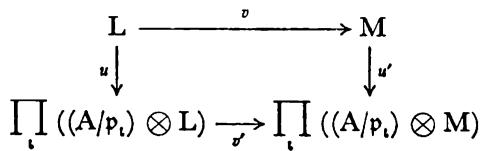
\includegraphics[keepaspectratio]{images/part001_964082be.jpg}}

其中 \(u\)（相应地 \(u'\)）是映射 \(x \mapsto (\phi_{\iota}(x))\)（相应地 \(y \mapsto (\psi_{\iota}(y)))\)），

\[
\phi_ {i} \colon \mathbf {L} \rightarrow (\mathbf {A} / \mathfrak {p} _ {i}) \otimes \mathbf {L}
\]

（相应地 \(\psi_{t}\colon\mathbf{M}\to(\mathbf{A}/p_{t})\otimes\mathbf{M}\)）是典范映射，而 \(v'\) 是诸 \(1_{\mathbf{A}/p_{t}}\otimes v\) 的乘积。于是 \((\mathbf{A}/p)/(m/p_{t})\otimes_{\mathbf{A}/p_{t}}((\mathbf{A}/p_{t})\otimes_{\mathbf{A}}\mathbf{M})=(\mathbf{A}/m)\otimes_{\mathbf{A}}\mathbf{M}\)，且由于 \(A/p_{t}\) 是局部整环，由论证的第一部分可得每个 \(1_{\mathbf{A}/p_{t}}\otimes v\) 都是同构；从而 \(v'\) 也是同构。另一方面，由于 A 是约化的，\(\bigcap_{i} p_{i} = (0)\)（\(\S 2\) 2 第 6 节命题 13），又因 L 是自由的，故 \(\bigcap_{i} (p_{i} L) = 0\)（《代数》第 II 章 \(\S 3\) 3 第 7 节注）；由于 \(p_{i} L\) 是 \(\phi_{i}\) 的核，这表明 \(u\) 是单射。由此推出 \(v' \circ u = u' \circ v\) 是单射，因而 \(v\) 是单射；而按定义 \(v\) 是满射，故这表明 M 是自由的。

